% =====================================================================
% ELMED219: Maskinlæring – grunnleggende konsepter (M01-M10)
% Beamer-presentasjon i widescreen (16:9)
% =====================================================================
\documentclass[aspectratio=169, 10pt]{beamer}

% =====================================================================
% PAKKER
% =====================================================================
\usepackage[utf8]{inputenc}
\usepackage[T1]{fontenc}
\usepackage[norsk]{babel}
\usepackage{graphicx}
\usepackage{tikz}
\usetikzlibrary{shapes.geometric, arrows, positioning, shapes.symbols}
\usepackage{booktabs}
\usepackage{amsmath}
\usepackage{fontawesome5}
\usepackage{hyperref}
\hypersetup{colorlinks=true, linkcolor=blue, urlcolor=blue}

% =====================================================================
% TEMA OG FARGER
% =====================================================================
\usetheme{Madrid}
\usecolortheme{beaver}

% Farger for TikZ-diagrammer
\definecolor{uibblue}{RGB}{0, 61, 115}
\definecolor{uibred}{RGB}{175, 28, 44}

% =====================================================================
% TITTELINFO
% =====================================================================
\title{Maskinlæring -- Grunnleggende konsepter}
\subtitle{ELMED219: Momentliste M01--M10}
\author{ELMED219}
\date{Vår 2026}

% =====================================================================
% DOKUMENT
% =====================================================================
\begin{document}

% ---------------------------------------------------------------------
% Tittelslide
% ---------------------------------------------------------------------
\begin{frame}
    \titlepage
\end{frame}

% ---------------------------------------------------------------------
% Oversikt
% ---------------------------------------------------------------------
\begin{frame}{Oversikt}
    \begin{enumerate}
        \item \textbf{Hva er maskinlæring?}
        \begin{itemize}
            \item M01: Definisjon og skille fra tradisjonell programmering
            \item M02: Supervised vs. Unsupervised læring
            \item M03: Features og Labels
        \end{itemize}
        \item \textbf{Validering og modelltyper}
        \begin{itemize}
            \item M04--M05: Trenings-/testsett, overtilpasning/undertilpasning
            \item M06--M07: Bias-Variance trade-off, K-fold kryssvalidering
            \item M08--M10: Baseline, klassifisering vs. regresjon, enkle modeller
        \end{itemize}
    \end{enumerate}
\end{frame}

% =====================================================================
\section{Hva er maskinlæring?}
% =====================================================================

% ---------------------------------------------------------------------
% M01
% ---------------------------------------------------------------------
\begin{frame}{M01: Definere \href{https://en.wikipedia.org/wiki/Machine_learning}{maskinlæring} og skille fra tradisjonell programmering}

    \begin{columns}
        \begin{column}{0.48\textwidth}
            \textbf{Tradisjonell programmering:}
            \begin{itemize}
                \item Eksplisitte regler definert av programmerer
                \item \texttt{if-else} logikk, deterministisk
                \item Input + Regler $\rightarrow$ Output
                \item Krever full domenekunnskap på forhånd
            \end{itemize}

            \vspace{2mm}
            \textbf{Maskinlæring:}
            \begin{itemize}
                \item Lærer regler fra data automatisk
                \item Mønstergjenkjenning, statistisk
                \item Input + Output $\rightarrow$ Regler (modell)
                \item Skalerer med datamengde
            \end{itemize}
        \end{column}

        \begin{column}{0.48\textwidth}
            \begin{block}{\scriptsize \href{https://www.cs.cmu.edu/~tom/mlbook.html}{Definisjon (Tom Mitchell, 1997)}}
                \scriptsize
                \textit{``A computer program is said to \textbf{\textit{learn from experience}} E with respect to some task T and some performance measure P, if its performance on T, as measured by P, improves with experience E.''}
            \end{block}

            \begin{block}{\scriptsize Definisjon (Tom Mitchell, 1997) -- på norsk}
                \scriptsize
                \textit{``Et dataprogram sies å \textbf{\textit{lære av erfaring}} E med hensyn til en oppgave T og et ytelsesmål P, dersom dets ytelse på T, målt ved P, forbedres med erfaring E.''}
            \end{block}
        \end{column}
    \end{columns}

\end{frame}

% ---------------------------------------------------------------------
% M02
% ---------------------------------------------------------------------
\begin{frame}{M02: \href{https://en.wikipedia.org/wiki/Supervised_learning}{Supervised} vs. \href{https://en.wikipedia.org/wiki/Unsupervised_learning}{Unsupervised} læring}

    \begin{columns}
        \begin{column}{0.48\textwidth}
            \textbf{\faCheckCircle\ Supervised (veiledet) læring:}
            \begin{itemize}
                \item Data har \textbf{labels} (fasit/merkelapper)
                \item Modellen lærer input$\rightarrow$output-mapping
                \item Typer: Klassifisering, regresjon
                \item Medisinsk: Diagnostisering, prognose
                \item Krever manuell annotering av data
            \end{itemize}
        \end{column}

        \begin{column}{0.48\textwidth}
            \textbf{\faSearch\ Unsupervised (ikke-veiledet) læring:}
            \begin{itemize}
                \item Data \textbf{uten} labels
                \item Finner skjulte mønstre/strukturer
                \item Typer: Klynging, dimensjonsreduksjon
                \item Medisinsk: Pasient-subgrupper
                \item Ingen fasit -- utforskende analyse
            \end{itemize}
        \end{column}
    \end{columns}

    \vspace{2mm}
    \begin{block}{\footnotesize \href{https://en.wikipedia.org/wiki/Semi-supervised_learning}{Semi-supervised} (delvis veiledet) -- prinsipper og anvendelser}
        \scriptsize
        Kombinerer få merkede eksempler med mange umerkede. Nyttig når annotering er dyrt/tidkrevende.\\[2pt]
        \textbf{Prinsipper:}
        \textit{Smoothness} -- nærliggende datapunkter har ofte samme label. \textit{Tabulært:} pasienter med like lab-verdier har ofte samme diagnose. \textit{Bilde:} MR-snitt med lignende pikselintensiteter viser lignende patologi.
        \textit{Cluster} -- data grupperer seg naturlig; punkter i samme klynge tilhører ofte samme klasse. \textit{Tabulært:} pasienter med diabetes klynger seg i feature-rommet. \textit{Bilde:} hjerne-MR av friske vs. Alzheimer danner separate klynger.
        \href{https://en.wikipedia.org/wiki/Manifold_hypothesis}{\textit{Manifold}} -- et 256$\times$256 bilde = 65536 piksler, men meningsfull variasjon bestemmes av få faktorer (anatomi, patologi). Bildene ``fyller'' ikke hele rommet, men ligger på en lavdim. flate.\\[2pt]
        \textbf{Anvendelser:} Medisinsk bildesegmentering, tekstklassifisering, talegjenkjenning, legemiddeloppdagelse, genomikk.
    \end{block}

\end{frame}

% ---------------------------------------------------------------------
% M03
% ---------------------------------------------------------------------
\begin{frame}{M03: \href{https://en.wikipedia.org/wiki/Feature_(machine_learning)}{Features} (input) og \href{https://en.wikipedia.org/wiki/Labeled_data}{Labels} (output)}

    \begin{block}{\footnotesize Definisjoner}
        \footnotesize
        \begin{itemize}
            \item \textbf{Features} ($\mathbf{X}$): Inputvariabler / egenskaper / kjennetegn som beskriver dataene
            \item \textbf{Labels} ($y$): Målvariabel / det vi ønsker å predikere (fasit)
        \end{itemize}
    \end{block}

    \vspace{2mm}
    \textbf{Eksempel -- Hjertesykdomsprediksjon (tabulære data):}

    \begin{table}
        \centering
        \footnotesize
        \begin{tabular}{cccc|c}
            \toprule
            \textbf{Alder} & \textbf{Kolesterol} & \textbf{Blodtrykk} & \textbf{BMI} & \textbf{Sykdom?} \\
            \midrule
            55 & 240 & 140 & 28 & Ja \\
            32 & 180 & 120 & 23 & Nei \\
            67 & 210 & 155 & 31 & Ja \\
            \bottomrule
        \end{tabular}
    \end{table}

    \begin{center}
        \footnotesize
        \textcolor{uibblue}{\textbf{Features} $\mathbf{X}$ (kolonner = variabler)} \hspace{1cm} \textcolor{uibred}{\textbf{Label} $y$}\\
        Rader = observasjoner/pasienter, Kolonner = variabler $\rightarrow$ \textbf{Matrise}
    \end{center}

\end{frame}

% ---------------------------------------------------------------------
% M04
% ---------------------------------------------------------------------
\begin{frame}{M04: Hvorfor \href{https://en.wikipedia.org/wiki/Training,_validation,_and_test_data_sets\#Training_data_set}{treningssett} og \href{https://en.wikipedia.org/wiki/Training,_validation,_and_test_data_sets\#Test_data_set}{testsett}?}

    \textbf{Problemet:} Hvordan vet vi om modellen generaliserer til nye data?

    \vspace{2mm}
    \begin{columns}
        \begin{column}{0.55\textwidth}
            \begin{block}{\footnotesize Løsningen: Data-splitting}
                \footnotesize
                \begin{enumerate}
                    \item Del datasettet i to (eller tre) deler
                    \item \textbf{Treningssett} ($\sim$70--80\%): Tren modellen
                    \item \textbf{Testsett} ($\sim$20--30\%): Evaluer på usett data
                    \item (Valideringssett: Tuning av hyperparametre)
                \end{enumerate}
            \end{block}
        \end{column}

        \begin{column}{0.4\textwidth}
            
\begin{tikzpicture}[scale=0.8]
                \fill[uibblue!60] (0,0) rectangle (4,1);
                \fill[uibred!60] (4,0) rectangle (5.5,1);
                \node[white] at (2, 0.5) {\small Trening (70\%)};
                \node[white] at (4.75, 0.5) {\small Test};
            \end{tikzpicture}
        \end{column}
    \end{columns}

    \vspace{2mm}
    \begin{columns}[T]
        \begin{column}{0.48\textwidth}
            \begin{alertblock}{\footnotesize Viktig}
                \footnotesize Modellen skal \textbf{aldri} se testdataene under trening!
            \end{alertblock}
        \end{column}
        \begin{column}{0.48\textwidth}
            \begin{block}{\footnotesize \href{https://scikit-learn.org/stable/modules/generated/sklearn.model_selection.train_test_split.html}{scikit-learn}}
                \footnotesize \texttt{train\_test\_split(X, y, test\_size=0.2)}
            \end{block}
        \end{column}
    \end{columns}

\end{frame}

% ---------------------------------------------------------------------
% M05
% ---------------------------------------------------------------------
\begin{frame}{M05: \href{https://en.wikipedia.org/wiki/Overfitting}{Overtilpasning (Overfitting)} og \href{https://en.wikipedia.org/wiki/Overfitting\#Underfitting}{Undertilpasning (Underfitting)}}

    \begin{columns}
        \begin{column}{0.32\textwidth}
            \textbf{Undertilpasning:}
            \begin{itemize}
                \item For enkel modell
                \item Høy bias
                \item Dårlig på trening og test
            \end{itemize}
            \begin{center}
                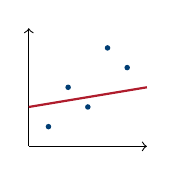
\begin{tikzpicture}[scale=0.5]
                    \draw[->] (0,0) -- (3,0);
                    \draw[->] (0,0) -- (0,3);
                    \fill[uibblue] (0.5,0.5) circle (2pt);
                    \fill[uibblue] (1,1.5) circle (2pt);
                    \fill[uibblue] (1.5,1) circle (2pt);
                    \fill[uibblue] (2,2.5) circle (2pt);
                    \fill[uibblue] (2.5,2) circle (2pt);
                    \draw[uibred, thick] (0,1) -- (3,1.5);
                \end{tikzpicture}
            \end{center}
        \end{column}

        \begin{column}{0.32\textwidth}
            \textbf{God tilpasning:}
            \begin{itemize}
                \item Riktig kompleksitet
                \item Balanse
                \item Generaliserer godt
            \end{itemize}
            \begin{center}
                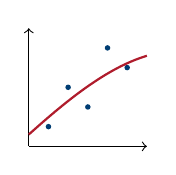
\begin{tikzpicture}[scale=0.5]
                    \draw[->] (0,0) -- (3,0);
                    \draw[->] (0,0) -- (0,3);
                    \fill[uibblue] (0.5,0.5) circle (2pt);
                    \fill[uibblue] (1,1.5) circle (2pt);
                    \fill[uibblue] (1.5,1) circle (2pt);
                    \fill[uibblue] (2,2.5) circle (2pt);
                    \fill[uibblue] (2.5,2) circle (2pt);
                    \draw[uibred, thick] (0,0.3) .. controls (1,1.2) and (2,2) .. (3,2.3);
                \end{tikzpicture}
            \end{center}
        \end{column}

        \begin{column}{0.32\textwidth}
            \textbf{Overtilpasning:}
            \begin{itemize}
                \item For kompleks modell
                \item Høy varians
                \item Lærer støy i dataene
            \end{itemize}
            \begin{center}
                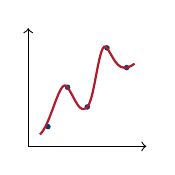
\begin{tikzpicture}[scale=0.5]
                    \draw[->] (0,0) -- (3,0);
                    \draw[->] (0,0) -- (0,3);
                    \fill[uibblue] (0.5,0.5) circle (2pt);
                    \fill[uibblue] (1,1.5) circle (2pt);
                    \fill[uibblue] (1.5,1) circle (2pt);
                    \fill[uibblue] (2,2.5) circle (2pt);
                    \fill[uibblue] (2.5,2) circle (2pt);
                    \draw[uibred, thick] (0.3,0.3) .. controls (0.6,0.6) and (0.8,1.8) .. (1,1.5) .. controls (1.2,1.2) and (1.3,0.8) .. (1.5,1) .. controls (1.7,1.2) and (1.8,2.8) .. (2,2.5) .. controls (2.2,2.2) and (2.3,1.8) .. (2.7,2.1);
                \end{tikzpicture}
            \end{center}
        \end{column}
    \end{columns}

    \vspace{3mm}
    \begin{block}{\footnotesize Kjennetegn på overtilpasning}
        \footnotesize Stor forskjell mellom trenings- og test-\href{https://en.wikipedia.org/wiki/Evaluation_of_machine_learning_models}{ytelse} (performance). \textbf{Ytelse} = mål på hvor godt modellen presterer (f.eks. accuracy, F1).
    \end{block}

\end{frame}

% ---------------------------------------------------------------------
% M06
% ---------------------------------------------------------------------
\begin{frame}{M06: \href{https://en.wikipedia.org/wiki/Bias\%E2\%80\%93variance_tradeoff}{Bias-Variance Trade-off}}

    \textbf{Totalt prediksjonsfeil:}
    \[ \text{MSE} = \underbrace{\text{Bias}^2}_{\text{systematisk feil}} + \underbrace{\text{Varians}}_{\text{tilfeldig feil}} + \underbrace{\sigma^2}_{\text{irreducible}} \]

    \vspace{1mm}
    \begin{columns}
        \begin{column}{0.48\textwidth}
            \textbf{Bias (systematisk feil):}
            \begin{itemize}
                \item Feil pga. forenklet modell
                \item Høy bias $\rightarrow$ \textbf{undertilpasning}
                \item Modellen ``misser'' mønsteret
            \end{itemize}

            \vspace{2mm}
            \textbf{Varians (tilfeldig feil):}
            \begin{itemize}
                \item Sensitiv for små endringer i data
                \item Høy varians $\rightarrow$ \textbf{overtilpasning}
                \item Modellen ``husker'' støy
            \end{itemize}
        \end{column}

        \begin{column}{0.48\textwidth}
            \begin{center}
                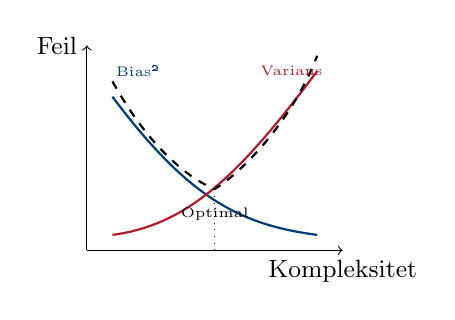
\begin{tikzpicture}[scale=0.65]
                    \draw[->] (0,0) -- (5,0) node[below] {\small Kompleksitet};
                    \draw[->] (0,0) -- (0,4) node[left] {\small Feil};

                    \draw[uibblue, thick] (0.5,3) .. controls (2,1) and (3,0.5) .. (4.5,0.3);
                    \draw[uibred, thick] (0.5,0.3) .. controls (2,0.5) and (3,1.5) .. (4.5,3.5);
                    \draw[black, thick, dashed] (0.5,3.3) .. controls (1.5,1.5) and (2.5,1.2) .. (2.5,1.2) .. controls (3,1.5) and (4,2.5) .. (4.5,3.8);

                    \node[uibblue] at (1, 3.5) {\tiny Bias²};
                    \node[uibred] at (4, 3.5) {\tiny Varians};
                    \node at (2.5, 0.7) {\tiny Optimal};

                    \draw[dotted] (2.5, 0) -- (2.5, 1.2);
                \end{tikzpicture}
            \end{center}
        \end{column}
    \end{columns}

    \begin{block}{\scriptsize Målet}
        \scriptsize Finn balansen som minimerer \textbf{total feil} på nye data. $\sigma^2$ = støy i data (kan ikke reduseres).
    \end{block}

\end{frame}

% =====================================================================
\section{Validering og modelltyper}
% =====================================================================

% ---------------------------------------------------------------------
% M07
% ---------------------------------------------------------------------
\begin{frame}{M07: \href{https://en.wikipedia.org/wiki/Cross-validation_(statistics)\#k-fold_cross-validation}{K-fold kryssvalidering}}
    
    \textbf{Problem:} Ett enkelt train/test-split kan gi tilfeldige resultater
    
    \vspace{3mm}
    
    \textbf{Løsning: K-fold Cross-Validation}
    \begin{enumerate}
        \item Del data i $k$ like store deler (``folds'')
        \item For hver fold: bruk den som test, resten som trening
        \item Gjennomsnitt av alle $k$ evalueringer
    \end{enumerate}
    
    \vspace{3mm}
    
    \begin{center}
        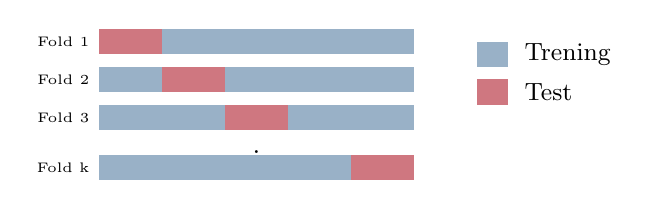
\begin{tikzpicture}[scale=0.8]
            % Fold 1
            \fill[uibred!60] (0,2) rectangle (1,2.4);
            \fill[uibblue!40] (1,2) rectangle (5,2.4);
            \node[left] at (0, 2.2) {\tiny Fold 1};
            
            % Fold 2
            \fill[uibblue!40] (0,1.4) rectangle (1,1.8);
            \fill[uibred!60] (1,1.4) rectangle (2,1.8);
            \fill[uibblue!40] (2,1.4) rectangle (5,1.8);
            \node[left] at (0, 1.6) {\tiny Fold 2};
            
            % Fold 3
            \fill[uibblue!40] (0,0.8) rectangle (2,1.2);
            \fill[uibred!60] (2,0.8) rectangle (3,1.2);
            \fill[uibblue!40] (3,0.8) rectangle (5,1.2);
            \node[left] at (0, 1) {\tiny Fold 3};
            
            % etc
            \node at (2.5, 0.4) {$\vdots$};
            
            \fill[uibblue!40] (0,0) rectangle (4,0.4);
            \fill[uibred!60] (4,0) rectangle (5,0.4);
            \node[left] at (0, 0.2) {\tiny Fold k};
            
            % Legend
            \fill[uibblue!40] (6, 1.8) rectangle (6.5, 2.2);
            \node[right] at (6.6, 2) {\small Trening};
            \fill[uibred!60] (6, 1.2) rectangle (6.5, 1.6);
            \node[right] at (6.6, 1.4) {\small Test};
        \end{tikzpicture}
    \end{center}
    
    \vspace{3mm}
    
    \textbf{Fordeler:} Mer robust estimat, bruker all data for både trening og testing
    
\end{frame}

% ---------------------------------------------------------------------
% M08
% ---------------------------------------------------------------------
\begin{frame}{M08: \href{https://en.wikipedia.org/wiki/Baseline_(machine_learning)}{Baseline-modell}}

    \begin{block}{\footnotesize Hva er en baseline?}
        \footnotesize En \textbf{enkel referansemodell} som vår ML-modell må slå for å være nyttig.
    \end{block}

    \vspace{2mm}
    \textbf{Eksempler på baselines:}

    \begin{itemize}
        \item \textbf{Klassifisering:} Prediker alltid majoritetsklassen
        \begin{itemize}
            \item Datasett med 90\% friske, 10\% syke $\rightarrow$ baseline accuracy = 90\%
        \end{itemize}
        \item \textbf{Regresjon:} Prediker alltid gjennomsnittsverdien
        \item \textbf{Tidsserie:} Bruk forrige verdi som prediksjon
    \end{itemize}

    \vspace{2mm}
    \begin{alertblock}{\footnotesize Hvorfor viktig?}
        \footnotesize
        90\% accuracy høres imponerende ut, men ikke hvis baseline er 90\%! Viser om ML tilfører \textbf{faktisk verdi}. Avslører ubalanserte datasett.
    \end{alertblock}

\end{frame}

% ---------------------------------------------------------------------
% M09
% ---------------------------------------------------------------------
\begin{frame}{M09: \href{https://en.wikipedia.org/wiki/Statistical_classification}{Klassifisering} vs. \href{https://en.wikipedia.org/wiki/Regression_analysis}{Regresjon}}

    \begin{columns}
        \begin{column}{0.48\textwidth}
            \textbf{\faThLarge\ Klassifisering:}
            \begin{itemize}
                \item Predikerer \textbf{kategorier/klasser}
                \item Diskrete utfall
                \item Eksempler:
                \begin{itemize}
                    \item Syk / Frisk
                    \item Kreft type A / B / C
                \end{itemize}
            \end{itemize}

            \vspace{2mm}
            \textbf{Evalueringsmetrikker:}
            \footnotesize
            \begin{itemize}
                \item \href{https://en.wikipedia.org/wiki/Accuracy_and_precision\#In_classification}{Accuracy}, \href{https://en.wikipedia.org/wiki/Precision_and_recall\#Precision}{Precision}, \href{https://en.wikipedia.org/wiki/Precision_and_recall\#Recall}{Recall}
                \item \href{https://en.wikipedia.org/wiki/F-score}{F1-score}, \href{https://en.wikipedia.org/wiki/Receiver_operating_characteristic}{AUC-ROC}
            \end{itemize}
        \end{column}

        \begin{column}{0.48\textwidth}
            \textbf{\faChartLine\ Regresjon:}
            \begin{itemize}
                \item Predikerer \textbf{kontinuerlige verdier}
                \item Numeriske utfall
                \item Eksempler:
                \begin{itemize}
                    \item Blodtrykk
                    \item Medikamentdosering
                \end{itemize}
            \end{itemize}

            \vspace{2mm}
            \textbf{Evalueringsmetrikker:}
            \footnotesize
            \begin{itemize}
                \item \href{https://en.wikipedia.org/wiki/Mean_squared_error}{MSE}, \href{https://en.wikipedia.org/wiki/Root-mean-square_deviation}{RMSE}, \href{https://en.wikipedia.org/wiki/Mean_absolute_error}{MAE}
                \item \href{https://en.wikipedia.org/wiki/Coefficient_of_determination}{R²} (forklart varians)
            \end{itemize}
        \end{column}
    \end{columns}

\end{frame}

% ---------------------------------------------------------------------
% M10
% ---------------------------------------------------------------------
\begin{frame}{M10: Enkle ML-modeller}

    \begin{columns}
        \begin{column}{0.32\textwidth}
            \textbf{\href{https://en.wikipedia.org/wiki/Decision_tree_learning}{Beslutningstre}:}
            \begin{itemize}
                \item Serier av ja/nei-spørsmål
                \item Lett å tolke
                \item Kan overtilpasse
            \end{itemize}
            \begin{center}
                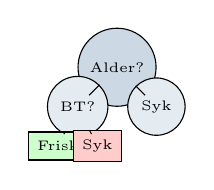
\begin{tikzpicture}[scale=0.5, every node/.style={font=\tiny}]
                    \node[draw, circle, fill=uibblue!20] (root) at (1.5,2) {Alder?};
                    \node[draw, circle, fill=uibblue!10] (l) at (0.5,1) {BT?};
                    \node[draw, circle, fill=uibblue!10] (r) at (2.5,1) {Syk};
                    \node[draw, rectangle, fill=green!20] (ll) at (0,0) {Frisk};
                    \node[draw, rectangle, fill=red!20] (lr) at (1,0) {Syk};
                    \draw (root) -- (l);
                    \draw (root) -- (r);
                    \draw (l) -- (ll);
                    \draw (l) -- (lr);
                \end{tikzpicture}
            \end{center}
        \end{column}
        
        \begin{column}{0.32\textwidth}
            \textbf{\href{https://en.wikipedia.org/wiki/K-nearest_neighbors_algorithm}{k-Nearest Neighbors}:}
            \begin{itemize}
                \item Finn $k$ mest like eksempler
                \item Majoritetsvotering
                \item Enkel, men treg
            \end{itemize}
            \begin{center}
                
\begin{tikzpicture}[scale=0.5]
                    \fill[uibblue] (0.5,0.5) circle (3pt);
                    \fill[uibblue] (0.8,1) circle (3pt);
                    \fill[uibblue] (1,0.7) circle (3pt);
                    \fill[uibred] (2,2) circle (3pt);
                    \fill[uibred] (2.3,1.8) circle (3pt);
                    \fill[uibred] (1.8,2.2) circle (3pt);
                    \node[draw, star, fill=green!50, scale=0.5] at (1.5,1.3) {};
                    \draw[dashed] (1.5,1.3) circle (0.6);
                \end{tikzpicture}
            \end{center}
        \end{column}
        
        \begin{column}{0.32\textwidth}
            \textbf{\href{https://en.wikipedia.org/wiki/Logistic_regression}{Logistisk regresjon}:}
            \begin{itemize}
                \item Lineær grense
                \item Gir sannsynligheter
                \item Rask og tolkbar
            \end{itemize}
            \begin{center}
                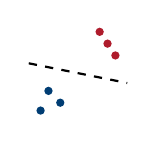
\begin{tikzpicture}[scale=0.5]
                    \fill[uibblue] (0.3,0.3) circle (3pt);
                    \fill[uibblue] (0.5,0.8) circle (3pt);
                    \fill[uibblue] (0.8,0.5) circle (3pt);
                    \fill[uibred] (2,2) circle (3pt);
                    \fill[uibred] (2.2,1.7) circle (3pt);
                    \fill[uibred] (1.8,2.3) circle (3pt);
                    \draw[thick, dashed] (0,1.5) -- (2.5,1);
                \end{tikzpicture}
            \end{center}
        \end{column}
    \end{columns}
    
    \vspace{5mm}
    
    \begin{block}{Tips}
        Start alltid med enkle modeller før du prøver komplekse!
    \end{block}
    
\end{frame}

% ---------------------------------------------------------------------
% Oppsummering
% ---------------------------------------------------------------------
\begin{frame}{Oppsummering: M01--M10}
    \vspace{-2mm}
    \begin{columns}
        \begin{column}{0.32\textwidth}
            \textbf{\footnotesize Nøkkelkonsepter:}
            \scriptsize
            \begin{itemize}\setlength{\itemsep}{0pt}
                \item ML lærer fra data
                \item Supervised / Unsupervised / Semi-supervised
                \item Features (X), Labels (y)
                \item Trening / test / validering
                \item Over-/undertilpasning
            \end{itemize}
        \end{column}
        \begin{column}{0.32\textwidth}
            \textbf{\footnotesize Beste praksis:}
            \scriptsize
            \begin{itemize}\setlength{\itemsep}{0pt}
                \item Kryssvalidering
                \item Sammenlign med baseline
                \item Klassifisering $\neq$ Regresjon
                \item Start enkelt
                \item Bias-varians-balanse
            \end{itemize}
        \end{column}
        \begin{column}{0.34\textwidth}
            \textbf{\footnotesize Fremtid: ML + GenAI}
            \scriptsize
            \begin{itemize}\setlength{\itemsep}{0pt}
                \item LLM-agenter for dataanalyse
                \item Multimodale modeller (tekst+bilde)
                \item RAG + kliniske retningslinjer
                \item Automatisert ML-pipeline
                \item Human-in-the-loop AI
            \end{itemize}
        \end{column}
    \end{columns}

    \vspace{0mm}
    \begin{block}{\scriptsize Medisinsk relevans -- ML-anvendelser i helse, medisin og bioteknologi}
        \scriptsize
        \textbf{Diagnostikk:} Bildediagnostikk (radiologi, patologi, oftalmologi, dermatologi), biomarkørdeteksjon, EKG/EEG-analyse.\\
        \textbf{Prognose:} Overlevelse (OS), progresjonsfri overlevelse (PFS), reinnleggelse, mortalitetsrisiko, sykdomsprogresjon.\\
        \textbf{Terapi:} Terapivalg, doseoptimalisering, behandlingsrespons, stråleplanlegging, kirurgisk navigasjon.\\
        \textbf{Legemiddel:} Drugability, målidentifikasjon, ADMET-prediksjon, virtual screening, de novo molekyldesign.\\
        \textbf{Helsesystem:} Ressursallokering, kapasitetsplanlegging, triagering, ventelisteoptimering, utbruddsdeteksjon.\\
        \textbf{Genomikk/biotek:} Variantklassifisering, genekspresjon, proteinstruktur (AlphaFold), single-cell, CRISPR off-target.\\
        \textbf{Psykiatri/nevrologi:} Stemningsanalyse, talemarkører, nevrodegenerasjon, anfallsprediksjon.\\
        \textbf{Folkehelse:} Epidemiologisk modellering, vaksinestrategi, sosiale determinanter, helseøkonomi (QALY/DALY).
    \end{block}
    
    \vspace{-1mm}
    \begin{center}
    \tiny\textbf{Human-in-the-loop:} Pasientbilde $\rightarrow$ \fbox{ML: ``mulig malign'' (87\%)} $\rightarrow$ Radiolog vurderer $\rightarrow$ Bekrefter/avviser $\rightarrow$ Feedback $\rightarrow$ Modell forbedres
    \end{center}

\end{frame}

\end{document}

